\documentclass[11pt,a4paper]{article}
\usepackage[german]{babel}
\usepackage[utf8]{inputenc}
\usepackage{bbm}
\usepackage{graphicx}
\usepackage{listings}
\usepackage{eufrak}


%%%%%%%%%% Start TeXmacs macros
\newcommand{\tmsamp}[1]{\textsf{#1}}
\newcommand{\tmtexttt}[1]{{\ttfamily{#1}}}
\newenvironment{tmindent}{\begin{tmparmod}{1.5em}{0pt}{0pt} }{\end{tmparmod}}
\newenvironment{tmparmod}[3]{\begin{list}{}{\setlength{\topsep}{0pt}\setlength{\leftmargin}{#1}\setlength{\rightmargin}{#2}\setlength{\parindent}{#3}\setlength{\listparindent}{\parindent}\setlength{\itemindent}{\parindent}\setlength{\parsep}{\parskip}} \item[]}{\end{list}}
\newenvironment{tmparsep}[1]{\begingroup\setlength{\parskip}{#1}}{\endgroup}
\newcommand{\extname}[1]{\mbox{\textbf{#1}}}
\newcommand{\bc}{\extname{bc }}
%%%%%%%%%% End TeXmacs macros

\author{Alexander Vogelgsang, Manuel Marschsll, Richard Sailer
\\
\\Lehrprofessur für Informatik, Universität Augsburg}
\title{Seminar: Bottom-up Datenverarbeitung auf der Unix Kommandozeile auch bekannt als Kommando Bimberle
\\Prozessbingo: Lottozahlen und Prozess-IDs}
\date{30.09.2014}

\begin{document}
\maketitle
\thispagestyle{empty}

\def\abstractname{Abstract.}
\begin{abstract}
Wir zeigen anhand des Fallbeispiels ``Prozessbingo: Lottozahlen und Prozess-ID's'' wie man mithilfe der \extname{BASH}, Textdaten  aus einer Website lesen und strukturiert weiterverarbeiten kann.
Außerdem werden wir aus Prozessnummern die maximal mögliche Menge an Enthropie gewinnen sowie daraus ein Sechstupel an Lottozahlen und eine Superzahl generieren.
\end{abstract}

\newpage
\thispagestyle{empty} 
\tableofcontents
\newpage

\section{Definitionen}
\label{sec:Definitionen}

Im Folgenden referenziert ``Lottoziehung'' ein 6 - Tupel $x = ( x_1, \ldots,
x_6)$ mit folgenden Eigenschaften:
\begin{enumerate}
  \item $\forall x_i, x_j \in x : x_i \neq x_j$ \ (In einer Ziehung kommt
  keine Zahl zwei Mal vor)
 
  \item $\forall x_i, x_j \in x : i < j \Rightarrow x_i, x_j$ \ (Die Tupel mit
  denen wir arbeiten sind sortiert)
\end{enumerate}

\section{Extraktion der Lottozahlen aus dem Archiv}

\subsection{Erste Überlegungen}

Um bestimmen zu können ob man jemals im Lotto gewonnen hätte, müssten die Lottozahlen erst in einem geeigneten Format zur Weiterverarbeitung vorliegen. Dazu wählen wir eine passende Internetseite. Wir entscheiden uns in diesem Fall für die Seite von ,,Lottozahlenonline'', weil die dort vorgefundenen Daten gut strukturiert sind und in Folge dessen einfach ausgelesen und die Jahre der Lottoziehungen durch einfache Anpassung der URL durchgeschaltet werden können.

\subsection{Arbeitsschritte}
Für jedes Jahr werden für die jeweilige Seite folgende Arbeitsschritte ausgeführt:

\begin{enumerate}
\item Herunterladen der Seite in eine temporäre Datei
\item Vorformatierung des HTML-Codes
\item Entfernen des unnötigen HTML-Codes
\item Extrahieren der Lottozahlen und des Datums in eine Tabelle
\item Nachformatierungen der extrahierten Daten und Speichern in temporäre Datei
\end{enumerate}

\begin{figure}[htbp]
  \centering
  \fbox{
    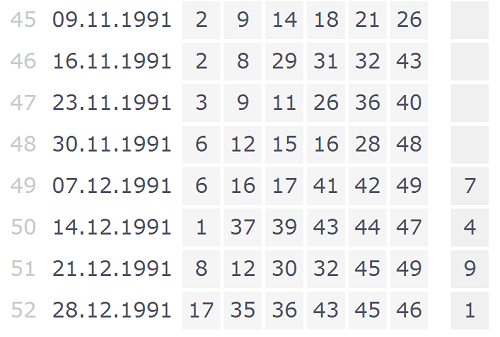
\includegraphics{page_big.png}
  }
  \caption{Aufbau der Internetseite. Man sieht folgende Daten (von links nach rechts): Nummer der Ziehung im Jahr, Datum der Ziehung und die dazugehörigen sechs Gewinnzahlen sowie Superzahl (falls vorhanden).}
  \label{page_header}
\end{figure}

Ist dieser Ablauf für jede Seite ausgeführt, werden alle Daten in einer Tabelle zusammengefasst. Die resultierende Datei liegt nun in dem schließlich gewünschten Format vor und es können relationale Anfragen darauf ausgeführt werden.
\newline
\newline
Wir nutzen nun allerdings das Tool \extname{wget}, um die Webseiten aus dem Internet herunterzuladen, da dieses verbreiteter zu sein scheint. Dazu bekommt \extname{wget} die URL der Seite, gefolgt von der jeweiligen Jahreszahl der Lottoziehung. Die Ausgabe wird in eine Datei mit ,,\$Jahreszahl.html'' geschrieben.
\newline
\newline
Um die spätere Verarbeitung zu vereinfachen, löschen wir Escape-Sequenzen aus dem Stream. Diese würden nämlich eine fehlerhafte Ausgabe hervorrufen und ihr Auftreten ist inkonsistent. Dazu nutzen wir \extname{tr}, das einzelne Zeichen löscht oder ersetzt. Dadurch ist es für diese Aufgabe perfekt geeignet.
\newline
\newline
Nun entfernen wir denjenigen Teil des HTML-Codes, der keine Beziehung zu den Lottozahlen aufweist. Dazu gehört alles bis auf die in Abbildung \ref{page_code} gezeigten Abschnitte. Wir benutzen dazu das Programm \extname{grep}. \extname{grep} dient dazu, mittels regulären Ausdrücken Text zu finden und die komplette Zeile des Textes auszugeben. Mit dem Parameter –o wird jedoch nur die gefundene Textpassage ausgegeben. Den verwendeten regulären Ausdruck zeigt Abbildung \ref{regex}.
\begin{figure}[htbp]
  \centering
  \fbox{
    \lstinputlisting[language=html,breaklines=true]{page_code.txt}
  }
  \caption{Page-Code}
  \label{page_code}
\end{figure}
\begin{figure}[htbp]
  \centering
  \fbox{
    \lstinputlisting{regular.txt}
  }
  \caption{Verwendeter regulärer Ausdruck. Dieser besteht aus vier Teilen. Der erste steht für die Ziehung, der zweite für das Datum der Ziehung, der dritte für die sechs Lottozahlen und der vierte für die Superzahl. Jeder dieser Teile hat die Form:
$<$div class="?"$>$???$<$/div$>$.
Der Inhalt der ,,divs'' stellt die zu extrahierenden Daten dar.
}
  \label{regex}
\end{figure}

Um die Daten tatsächlich in tabellarischer Form zu erhalten, löschen wir mithilfe des Programms \extname{sed} den HTML-Teil des verbleibenden Codes. Übrig bleiben die durch Leerzeichen getrennten Lottozahlen inklusive Datum und Ziehungsnummer. Dies erreichen wir durch den Substitutionsbefehl von sed. Mit diesem ersetzen wir die inneren divs durch Leerzeichen sowie das erste und letzte durch nichts. Das Ergebnis dieser Ausgabe zeigt Abbildung \ref{regex}.\newline
\newline
Schließlich fügen wir einen Stellvertreterwert für alle Ziehungen hinzu, in denen keine Superzahl gezogen wurde. Dies geschieht aus Konsistenzgründen.
\begin{figure}[htbp]
  \centering
  \fbox{
    \lstinputlisting{values.txt}
  }
  \caption{Resultierende Tabelle. Man sieht die Daten liegen wie in Abbildung \ref{page_code} vor, aber im Textformat.}
  \label{values}
\end{figure}

\subsection{Anpassungen}
Im endgültigen Programm vergleichen wir Lottozahlen zum einen mit der Superzahl, zum anderen ohne Superzahl mit unseren generierten Lottozahlen. Dazu erstellen wir zwei verschiedene Tabellen, einmal ohne Zusatz und einmal mit. Hierfür ist unser Stellvertreterwert sehr hilfreich, weil man mit ihm alle Ziehungen auswählen kann, die keine Superzahl beinhalten. Hierfür nutzen wir eine Kombination aus \extname{grep} und \extname{cut}. \extname{grep} extrahiert alle Zahlen mit beziehungsweise ohne Superzahl und \extname{cut} entfernt unnötige Spalten. In unserem Fall sind das die Ziehungsnummer und eventuell die Superzahl. Anschließend werden die Ergebnisse in zwei unterschiedliche Textdateien exportiert.


\section{Die Generierung der Lottozahlen aus den Prozess-IDs}

Die Menge der Prozess-IDs (im Folgenden PIDs) ist eine Menge $\mathbbm{P}$ aus natürlichen Zahlen.

Die Spezifikationen für das {\tmsamp{generate\_pid\_lottotips.sh}} Skript sind also aus der gegebenen Instanz von $\mathbbm{P}$, ein 6 - Tupel $x$ zu erzeugen, sodass die oben genannten Bedingungen erfüllt sind und außerdem noch eine weitere Superzahl zu generieren.
Des Weiteren haben wir uns das Ziel gesetzt, dies in einer Art zu tun, die:
\begin{enumerate}
  \item die komplette in $\mathbbm{P}$ enthaltene Enthropie nutzt.
  
  \item zuverlässig (unabhängig von $| \mathbbm{P} |$, somit der Anzahl der
  Prozesse auf dem System zum aktuellen Zeitpunkt) funktioniert.
  
  \item performant ist; (insofern dies mit einem \extname{Shellskript} möglich ist).
\end{enumerate}
Um Vergleichszahlen zu erhalten, generieren wir unsere eigenen Lottozahlen anhand der Prozess-ID's.
{\tmsamp{generate\_pid\_lottotips.sh}} erfüllt die Spezifikation.

\subsection{Das Programm (\tmtexttt{}generate\_pid\_lottotips.sh)}

Wir simulieren das normale Vorgehen einer Lottoziehung aus einer Trommel, aufgrund dessen diese Mthode programmiertechnisch gesehen die am einfachsten zu implementierende Lösung ist, die doppelte Lottozahlen verhindert und damit Definition \ref{sec:Definitionen} genügt.
Wir generieren uns ein Array \extname{lotto\_balls}, der die Trommel darstellt.
Aus diesem ziehen wir zufällig und hintereinander sechs Zahlen.
Der Zufall wird aus den \extname{PID's} berechnet.


Zuerst nehmen wir alle \extname{PID's},wobei uns das \extname{ps} Kommando hilft, und konkatenieren sie zu einem großen String.
Anschließend hashen wir diesen String mit der Hashfunktion \extname{sha512}. Nun werden alle Kleinbuchstaben a - f in Großbuchstaben A - F umgewandelt. Dies dient einer erleichterten Weiterverarbeitung. Als Nächstes wandeln wir diese Hexadezimalzahl mit dem Kommandozeilenrechner \bc in eine dezimale Zahl um.
Für \bc haben wir uns entschieden, weil dieses Werkzeug hervorragend mit extrem großen Zahl umgehen kann, da es die GNU BigNumberLibrary verwendet, im Gegensatz zu der in der BASH eingebauten \extname{Arithmetic Evaluation}.

Gesetzt wurde die Variable ibase, um bc zu sagen welche Basis die über STDIN erhaltenen Zahlen haben. Die Verwendung der Variablen ibase und obase ist ein unter UNIX Nutzern beliebter Trick zur schnellen Umwandlung zwischen beliebigen Zahlensystemen auf der Kommandozeile. Da die Ausgabe Basis das Dezimalsystem ist (default) muss obase hier nicht angepasst werden.

Abbildung \ref{balltopick} zeigt welche Bälle später aus dem Array \extname{lotto\_balls} gezogen werden.

\begin{figure}[htbp]
  \centering
  \fbox{
    \lstinputlisting{balltopick.txt}
  }
  \caption{Hier benutzen wir die \extname{Arithmetic Evaluation} und die Stringbearbeitungsfeatures der \extname{BASH}. \$(var:a:b) selektiert b-Zeichen aus der Stringvariable var von der Stelle a ab. \$(()) führt eine \extname{Arithmetic Evaluation Enviroment}  ein. Deswegen funktionieren die Rechenoperationen \extname{\%} und \extname{+}. Das Sigel 10\# vor dem \$-Sigel ist notwendig, um zu verhindern, dass die \extname{BASH} Zahlen, die mit einer führenden 0 beginnen, als Oktalzahl interpretiert werden und das Programm damit bei Zahlen wie 08 und 09 Fehlermeldungen ausgibt und damit terminiert.}
  \label{balltopick}
\end{figure}

Da \extname{lotto\_balls} mit jeder Ziehung um eine Zelle kleiner wird, ist auch die obere Schranke für die Indizes (der Divisor unserer Modulooperation)
  \extname{ball\_to\_pick} für jede Ziehung um 1 kleiner gewählt.

Aus Performance Gründen haben wir uns hier, genause wie bei den String Operationen der vorherigen Schritte, dafür entschieden, möglichst viel über die bash internen Operatoren (bzw. hier die Arithmetik Evaluation Erweiterung der \extname{BASH}) zu arbeiten.
Dies ist gegenüber dem Aufruf von externen Programmen, die extra von der Festplatte oder aus einem Cache geladen werden müssen deutlich effizienter.

Die Extraktion der Superzahl aus dem hashed \extname{PID} String verläuft auf ähnliche Art und Weise.

Im Folgenden nehmen wir aus der Tombola, simuliert durch das Array \extname{lotto\_balls}, sechs Zahlen.

Dies funktioniert genauso wie bei einer echten Tombola. Nachdem ein Element gezogen wurde, wird es aus dem Array entfernt.

Zuletzt werden die Lottozahlen in einen String überführt, der diese in sortierter Reihenfolge enthält (die Sortierung wird über GNU Sort mit Parameter -n erreicht).

Dies ist notwendig um die Suche nach einem Treffer in den Archivlottozahlen effizient und performant umzusetzen, da die Lottozahlen dort auch in sortierter Reihenfolge vorliegen.

\section{Überprüfung auf Gewinnkombinationen und eine Benutzerschnittstelle}

Wir haben nun sowohl die Archivzahlen als auch unsere im vorherigen Abschnitt erstellte Lottoziehung $\mathfrak{L}$.

In der Datei \extname{mainbusinesslogic.sh} suchen wir mithilfe von grep in den Archivlottozahlen nach $\mathfrak{L}$.

Eine erfolgreiche Suche bedeutet, dass unser $\mathfrak{L}$ in den Archivlottozahlen vorkommt und wir mit $\mathfrak{L}$ im Lotto gewonnen hätten.

Der Zeitpunkt dieses spekulativen Lottogewinns wird zusammen mit anderen wertvollen Informationen über die Whiptail Benutzerschnittstelle in einer ansprechenden modernen und zeitgemäßen Form ausgegeben.

\section{Fazit}
In diesem Seminar haben wir die \extname{BASH} und die Kommandozeilentools kennengelernt und daher vor allem wie man mit ihnen Daten, insbesondere Text in strukturierter Form, verarbeitet.
Insgesamt sind wir zu dem Schluss gekommen, dass die BASH mit dazugehörigen POSIX-Programmen für diesen Zweck nur mittelmäßig gut geeignet sind. \extname{Perl} wurde für genau diesen Zweck geschaffen und erlaubt für den Programmierer deutlich angenehmere und effizientere Möglichkeiten der Datenverarbeitung.
Die Datenstrukturen und Datentypen in \extname{BASH} sind wenig umfangreich und in Hinblick auf ihre Möglichkeiten nur eingeschränkt nutzbar. So können Funktionen zum Beispiel keine Arrays zurückgeben. Außerdem integriert der Array-Datentyp nur auf sehr plumpe Art und Weise mit externen Programmen und Build-In Methoden. Oftmals muss mit einer for-Schleife über alle Elemente interiert werden, bei Tätigkeiten, für die \extname{Perl} sehr viel angenehmer zu benutzende Build-In Methoden bietet.
Außerdem ist die Syntax schwierig zu durchschauen, da sie sehr vom Kontext abhängig ist. So ist es im Gegensatz zu vielen anderen Sprachen durchaus wichtig, an welcher Stelle man ein Leerzeichen setzt und an welcher nicht.
Abschließend lässt sich sagen, dass es sicherlich einige Anwendungsfälle gibt, für die Shell-Skript gut geeignet ist, wie zum Beispiel Automatisierung von Administrationsaufgaben oder das Arbeiten mit Dateien, komplexere Textverarbeitungsaufgaben gehören jedoch nicht dazu. Wir hatten viel Spaß am Kommando Bimberle xD.
\end{document}